\section{GNN models overview}
\label{sec:models}



In this section, we will provide a short literature review from the first attempts to
apply neural nets to graph data to modern approaches using using convolutions and attention mechanism.


% GNN

Early attempts to adapt neural network architectures to operate with graph data 
were proposed in works \cite{FirstGNN1} and  \cite{FirstGNN2}. These models 
used recursive neural networks (RNN) architecture. However these methods could be applied
only to directed acyclic graphs, which led to a serious restriction in their usage.
Models known as Graph Neural Networks (GNNs) were propesed in  \cite{GNNlist1}, \cite{GNNlist2}, \cite{GNN}.
These models generalized recursive neural networks to deal with more general classes of graphs.
Presented in \cite{GNN} GNN architecture is commonly refered as vanilla GNN.


Over the last decade, there have been proposed a huge number of new architectures and frameworks, which 
outperform vanilla GNNs. Below there will be desctibed several of them. 

% GCN


One of the most common modern approaches to constructing of graph neural network is
neural networks based on convolutions.

Convolution based neural networks (CNNs) have been applied to a wide range of computer
vision tasks and have proved their effectiveness to operate with grid-like structure data, such as images.
This approach has been proposed in \cite{CNN}.

Any grid can be seen as a graph of grid like structure in the Euclidean space. So the idea to extend and generalize
convolutions to graph data seemed to be very natural and aroused great interest among researchers.


Convolution used in CNNs has predefined reception field. Which means, that convolution kernel is 
applied to the neighbourhood of predefined size. In case of grid-like structure data, such as
images, the structure of the image doesn't change: each pixel has same number of neighbors. 
However, such property is not guaranteed for graph data. Each node of the graph may have 
different number of neighbors, so neighbourhood structure differs from node to node. So,
to apply convolutions to graph data, it should be prepared to operate with neighborhood 
with different structure.

\begin{figure}[t]
    \centering
    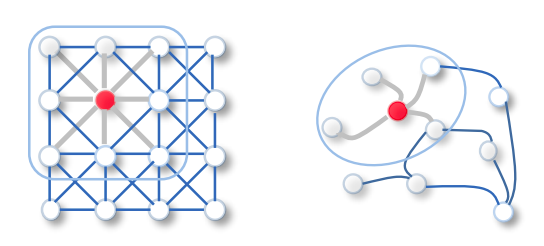
\includegraphics[width=1\textwidth]{conv_vs_grpahconv}
    \caption{2D Convolution vs. Graph Convolution \cite{SurveyOnGNN}}
    \label{fig:conv}
\end{figure}

The first solution of this problem was proposed in Spectral Network model \cite{Spectral}.This work proposes
to define convolution operation on graphs using eigendecomposition of the graph Laplacian.

For a undirected graph $G = (V,E)$ with $|V|=n$ , graph Laplacian matrix  $L \in \mathbb{R}^{n \times n}$ is defined as 

\begin{equation}
    L = D - A
    \label{eq:laplacian}
 \end{equation}

where $A$ is adjacency matrix of the graph, and $D$ is degree matrix.

Adjacency matrix $A \in \mathbb{R}^{n \times n}$ contains information about graph structure and is defined as:

\begin{equation}
    A_{ij} = 
    \begin{cases}
        1 \text{ if } \{v_i, v_j \} \in E, i \neq j,\\
        0 \text{ otherwise},\\
    \end{cases}
    \label{eq:adj}
\end{equation}

Degree matrix $D \in \mathbb{R}^{n \times n}$ is a diagonal matrix containing degrees of vertices and defined as:

\begin{equation}
    D_{ii} = deg(v_i)
    \label{eq:deg_mat}
 \end{equation}


Symmetic normalized Laplacian is defined as 

\begin{equation}
    L = D^{-\frac{1}{2}}LD^{-\frac{1}{2}} = I - D^{-\frac{1}{2}}AD^{-\frac{1}{2}}
    \label{eq:normalized_laplacian}
 \end{equation}

\begin{figure}[t]
    \centering
    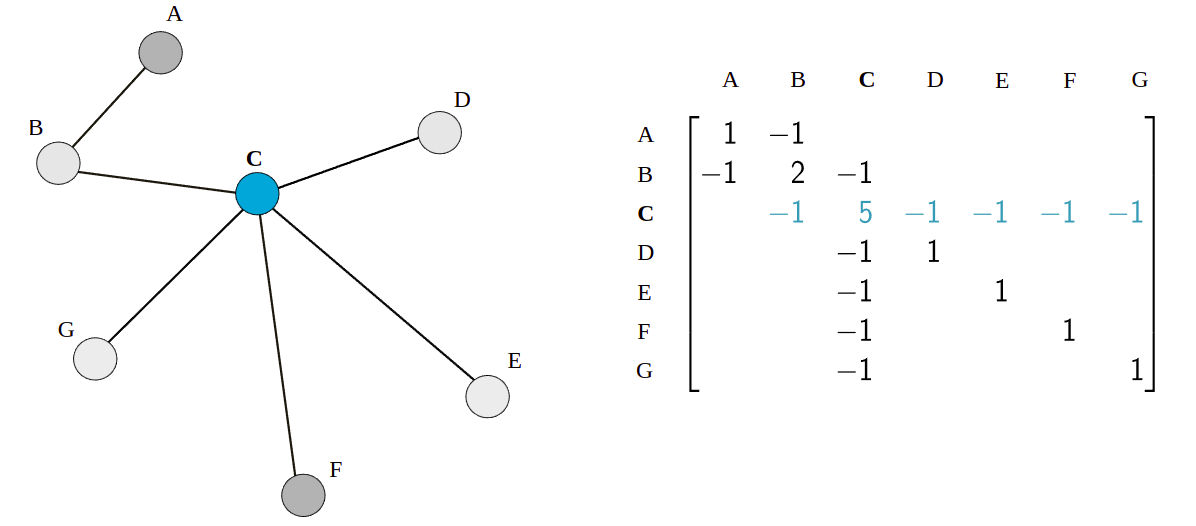
\includegraphics[width=0.7\textwidth]{laplacian}
    \caption{The example of Laplacian for a graph from \cite{distillGCN}}
    \label{fig:laplacian}
\end{figure}

The convolution operation  as for a feature node vector $x \in \mathbb{R}^N$ with a
filter $g_\theta = diag(\theta)$ parameterized by $\theta \in \mathbb{R}^N$ is defined as:


\begin{equation}
    Conv(g_\theta,x) = Ug_\theta(\Lambda)U^{T}x
    \label{eq:simple_conv}
 \end{equation}


where $U$ is the matrix of eigenvectors of the normalized Laplacian, $\Lambda$ is a diagonal matrix of 
eigenvalues from the spectral decomposition of normalized Laplacian: $L = I - D^{-\frac{1}{2}}AD^{-\frac{1}{2}} = U\Lambda U^{T}$.

Such approach to the definition of convolution on graph data is known as localized spectral filter. And used convolutions is known as 
spectral convolutions.
However, this convolution operation is very computational expensive as multiplication with matrix $U$ has complexity $O(n^2)$.


Authors of \cite{ChebAppr} susuggested to use approximation to calculate 
$Conv(g_\theta,x)$ using Chebyshev polinomials $T_k(x)$ up to $K^{th}$, which is defined as 

\begin{equation}
    T_k (x) = 2xT_{k-1}(x) - T_{k-2}(x)
    \label{eq:cheb_polynom}
 \end{equation}


where $T_0(x)=1$ an $T_1(x)=x$

So convolution of a signal $x$ with filter $g_\theta$ is suggested to be:

\begin{equation}
    Conv(g_\theta,x) \approx \sum_{k=0}^{K}{\theta}_k T_k(\hat{L})x
    \label{eq:conv_appr}
 \end{equation}

where $\hat{L} = \frac{2}{\lambda_{max}}L-I_N$ and $\lambda_max$ 
stands for the largest eigenvalue of $L$.
The complexity of evaluating convolution in proposed way is $O(|E|)$, i.e. is linear in the number of edges.

In \cite{ChebNet} there was proposed ChebNet - a convolutional neural network on grpahs based on K-localized convolution.

Authors \cite{GCN} developed the idea of usage spectral convolution and presented GCN model. The key idea is to build
convolutional neural network by stacking multiple simplified convolution layers with limited parameter $K=1$.
Single layer of such network can be expressed as: 

\begin{equation}
    Conv(g_\theta,x) \approx {\theta}_0 T_0(\hat{L})x + {\theta}_1 T_1(\hat{L})x = {\theta}_0 x + {\theta}_1 (\frac{2}{\lambda_{max}}L-I_N)x
    \label{eq:gcn_conv_appr}
 \end{equation}

Then authors of \cite{GCN} suggested to approximate $\lambda_{max} \approx 2$, so the expresion turns into the following one:

\begin{equation}
    Conv(g_\theta,x) \approx {\theta}_0 x + {\theta}_1 (L-I_N)x = {\theta}_0 x - {\theta}_1 D^{-\frac{1}{2}}AD^{-\frac{1}{2}}x
    \label{eq:gcn_conv_appr2}
 \end{equation}

However, instead of two parameters $\theta_0$ and $\theta_1$ authors suggested to use the single one - $\theta = \theta_0 = -\theta_1$. Thus it allows to
address overfitting problem and to simplify computations per layer. So, the follwoing expression is


\begin{equation}
    Conv(g_\theta,x) \approx {\theta}(I_N + D^{-\frac{1}{2}}AD^{-\frac{1}{2}})x
    \label{eq:gcn_conv_appr3}
 \end{equation}

Such expression of the convolution operation has a flow. The multiplier  $D^{-\frac{1}{2}}AD^{-\frac{1}{2}}$ has eigenvalues in 
range $[0,2]$, so that it leads to numerical instabilities when its repeated applying as layers in neural network. To alleviate this
problem, authors propose to replace numerical unstable multiplier $D^{-\frac{1}{2}}AD^{-\frac{1}{2}}$
with $\tilde{D}^{-\frac{1}{2}}\tilde{A}\tilde{D}^{-\frac{1}{2}}$, where $\tilde{A}=A+I_N$ and $\tilde{D}_{ii}=\sum_{j}\tilde{A}_{ij}$.

The final rule for linear convolutional layer for GCN can be generalized as following. Let signal $X \in \mathbb{R}^{N\times C}$ is a matrix of $C$-dimensional
feature vectors for each of $N$ nodes, and $\Theta \in \mathbb{R}^{C \times F}$ is a matrix of filter parameters. So convoled signal $X' \in \mathbb{R}^{N \times F}$ is 
expessed as 

\begin{equation}
    X' = \tilde{D}^{-\frac{1}{2}}\tilde{A}\tilde{D}^{-\frac{1}{2}}X\Theta
    \label{eq:final_gcn}
\end{equation}

So, GCN model allows to calculate node representations as vectors (embeddings) using layer-wise convolutional neural network.

We can rewrite the equation \ref{eq:final_gcn} in term of neural network layer. So, obtained the graph convolutional layer 
is the following:

\begin{equation}
    H^{(l+1)} = ReLU(\tilde{D}^{-\frac{1}{2}}\tilde{A}\tilde{D}^{-\frac{1}{2}}H^{(l)}W^{(l)})
    \label{eq:final_gcn_nn}
\end{equation}

where $H^{(l)} \in \mathbb{R}^{n \times d}$ is a hidden state matrix on layer $l$, $d$ is a dimension
of the convolution and $W^{(l)} \in \mathbb{R}^{d \ time d}$ is a matrix of trainable parmeters of the layer $l$.

ReLU function is an activation function, used to add non-linearity to neural network layer. It is defined as

\begin{equation}
    ReLU(x) = max(0,x)
    \label{eq:relu}
\end{equation}

% GAT

Along with spectral convolution approach, there are other ways to prepare node embeddings. One of such approaches, is 
attention-based architecture model called Graph Attention Networks (GAT) proposed in \cite{GAT}.
The main idea of this model is to apply attention mechanism to graph data. Based on attention models have become 
the most common solution for many sequence-based tasks \cite{GATintro1}, \cite{GATintro2}.
The main feature of attention mechanism is that it allows to focus on the most relevant parts of the input 
to make a desicion.

Authors of \cite{GAT} proposes a graph attentional layer, which is a building block for the arbitrary graph atteniton network.
The input of the layer is a set of node feature $ h=\{ h_1,\dots , h_N \}$, where $h_i \in \mathbb{R}^F$, $N$ - number of nodes, $F$ - the number
of node features. As result of layer processing is a new set of node features with other dimension: $h' = \{ h'_1 \dots h'_N \}$.
Each layer computes attentions coefficients $\alpha_{ij}$ by applying attention mechanism function $\alpha : R^{F'} \times R^{F'} \rightarrow R$.
to input node features multiplied to the shared weight matrix $W \in \mathbb{R}^{F'} \times R^{F}$:

\begin{equation}
    e_{ij} = \alpha(Wh_i, Wh_j)
    \label{eq:att_coeff}
\end{equation}

This coefficient indicates the importance of of node j's features to node i. The next step is performing masked attention to 
be able to compute only coefficients for a node is some defined node's neighborhood $N$ and normalizing coefficients by neighborhood:

\begin{equation}
   \alpha_{ij} = softmax_j(e_{ij}) = \frac{exp(e_{ij})}{\sum_{k \in N_i}exp(e_{ik})}
\end{equation}

The last element is an attention function $\alpha$ itself. Authors of \cite{GAT} proposed to use
single-layer feedforward neural network parameterized by $a \in \mathbb{R}^{2F'}$ and apply LeakyReLU nonlinearity.

As a result, the coefficients computed by the attention mechanism can be expressed as
\begin{equation}
    \alpha_{ij} = \frac{exp(LeackyReLU(a^{T}[Wh_i || Wh_j]))}{\sum_{k \in N_i}LeackyReLU(a^{T}[Wh_i || Wh_k])}
    \label{eq:final_att_coef}
 \end{equation}

where $||$ denotes concatenation operation. LeackyReLU - a activation function similar to ReLU defined in \ref{eq:relu}, but
apable of taking negative values:

\begin{equation}
    LeackyReLU(x) = 
    \begin{cases}
        x, \text{ if } \geq 0, \\
        ax, \text{ otherwise} \\
    \end{cases}
    \label{eq:leacky_relu}
\end{equation}

When coefficients are obtained - we can apply them to corresponding nodes:

\begin{equation}
    h'_i = \sigma \left( \sum_{j \in {N_i}} \alpha_{ij} W h_j \right)
    \label{eq:final_att}
 \end{equation}

To stabilize training procedure, authors extends self-attention mechanism
to multi-head attention, proposed in \cite{AttentionIsAllYouNeed}.
The idea of multi-head attention is to train several representations for each nodes at the same layer. And the final embedding
is just a concatenation of the all produced ones. For $K$ independant heads  there is a following final representation of the node:

\begin{equation}
    h'_i = ||_{k=1}^{K}  \sigma \left( \sum_{j \in {N_i}} \alpha^{k}_{ij} W^{k} h_j \right)
    \label{eq:multihead}
\end{equation}

On the prediction (final) layer, instead of concatenation, authors suggest to employ averaging over all attention heads:

\begin{equation}
    h'_i =  \sigma \left( \frac{1}{K} \sum_{k=1}^{K} \sum_{j \in {N_i}} \alpha^{k}_{ij} W^{k} h_j \right)
    \label{eq:multihead2}
\end{equation}


This last step is called aggregation and show on image \ref{fig:gat}.

\begin{figure}[t]
    \centering
    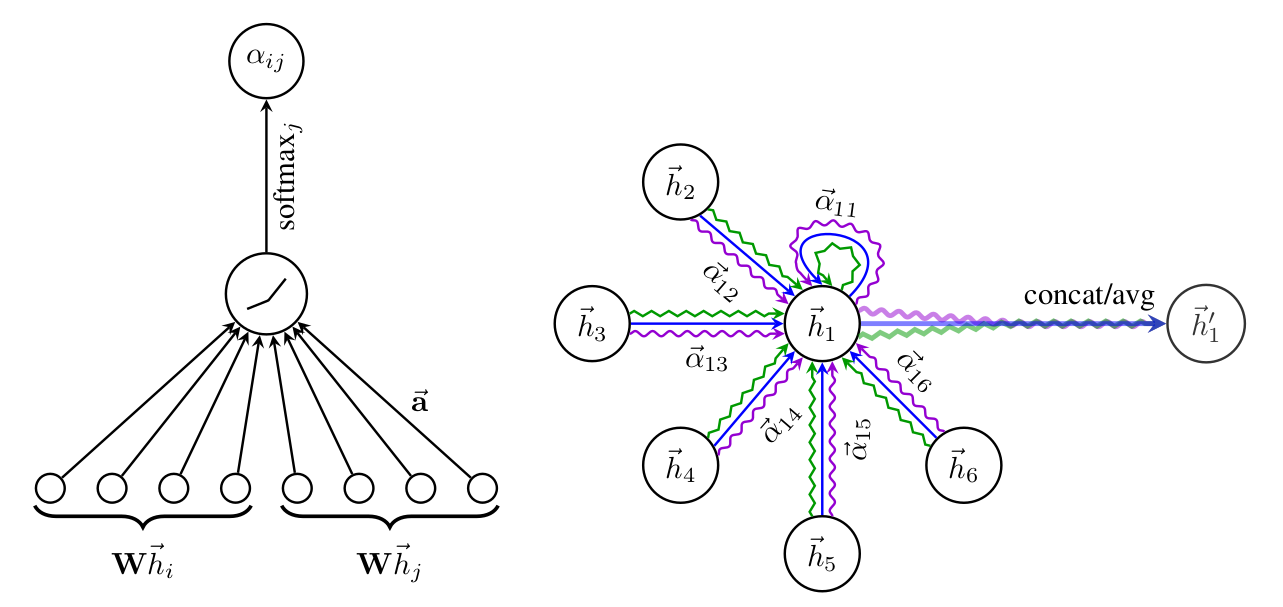
\includegraphics[width=0.7\textwidth]{gat}
    \caption{GAT network illustration from \cite{GAT}. Left: calculating of attention for each node. Right: feature aggregation from 3 head attention.}
    \label{fig:gat}
\end{figure}


So, GAT model allows to assign different importances to nodes of a same neighborhood which distinguishes it favorably from GCNs
model. Besides GAT model has another feature: the computation of the node-neighbor pairs is parallelizable thus the operation
of attention calculating is very efficient.

% GCN2

Both GCN\cite{GCN} and GAT\cite{GAT} models are shallow. Attempts to stacking more layers and to add non-linearity
tends to degrade the performance of these models \cite{GCNII} because of over-smoothing phenomena, described in \cite{OverSmoothing}.
Over-smoothing suggests that node representations becomes indistinguishable as thaey are inclined to converge 
to a certain value. This fact assigns restrictions on the number of layers in the network and as a result
limitations network's ability to extract information from high-order neighbors.


Authors of \cite{GCNII} extend GCN model with two modifications to prevent over-smoothing issue. Proposed architecture 
called Graph Convolutional Network via Initial residual and Identity mapping (GCNII).

The $l$-th layer of GCNII is defined as the following:

\begin{equation}
    H^{l+1} = ReLU\left( ((1-\alpha_{l})\tilde{P}H^{l} + \alpha_{l}H^{0}) ((1-\beta_{l})I_n + \beta_{l} W^{l})  \right)
    \label{eq:gcnii_layer}
\end{equation}

where $\alpha_l$ and $\beta_l$ are hyperparameters.
and $\tilde{P} = \tilde{D}^{-\frac{1}{2}}A\tilde{D}^{-\frac{1}{2}}$ is the graph 
convolution matrix with the renormalization trick used in equation \ref{eq:final_gcn} inside the GCN's layers.

Comparing with GCN layer defined in \ref{eq:final_gcn_nn} GCNII has two modifications.
The first one is to add initial residual connection to the first layer $H^0$. It simulates 
residual connections between different layers of the network originally proposed in 
ResNet model \cite{ResNet} in the filed of computer vision. 
The initial residual connection in GCNII ensures that that the final representation
of each node retains at least a fraction of $\alpha$ from the input layer even if the network contains
many layers stacked. Authors of \cite{GCNII} suggest to set hyperparameter $\alpha_l = 0.1$ or $0.2$.


The second modification is to add identity mapping $I_n$ to each layer's matrix of weights.
Adding of identity mapping provides regularization on weight matrix $W^{(l)}$ to avoid over-fitting.
The value of $\beta$ depends of the number of the layer. Authors suggest to set $\beta_l = \log(\frac{\lambda}{l}+1) \approx \frac{\lambda}{l}$,
where $\lambda$ is hyperparameter. 


% Pooling

Originally, GCN, GAT and GCNII models were developed for solving node classification problem.
These methods allows to get node embedding and learn neural network to match it to the specified label.

However, all these methods can be easily applied for solving graph classification problem using pooling operation \cite{distillGCN}.
Pooling operation allows to aggregate information from final node embeddings and the apply predictor for final graph classification.
In this work as aggregation function simple mean pooling function will be used:

\begin{equation}
    r_i = \frac{1}{N_i}\sum_{n=1}^{N_i}x_n
    \label{eq:mean_pool}
\end{equation}

where embedding vector $r_i$ of graph $i$ is calculated as a maen of node embeddings $x_n$.

As a final classifier, simple 2-layer perceptron will be used:
\begin{equation}
    c_i = W_2(Relu(W_1r_i))
    \label{eq:final_classifier}
\end{equation}


In the current paper the folowing models will be trained and evaluated: GCN\cite{GCN}, GAT\cite{GAT} and GCNII\cite{GCNII}.